%\documentclass[document.tex]{subfiles}
%\begin{document}

%%{\section{The Purpose of the Project}\label{sec:Purpose}}
\subsection{Purpose of the project}
\edcomm{YS}{Added the ``AMMBR section'' based on comments from Dr. Kahl. He has verified the section, I'll follow up with a proof read and other section of this document}

Ampersand follows a \emph{rule based} design principle. Rules are integral to an organization
and these are based on some principles and guidelines set by the organization.
Ampersand uses an ECA ( Event - Condition - Action) approach to make sure all rules are satisfied. An ideal information infrastructure supports employees and other stakeholders to maintain the rules of the business. To maintain a rule means to prevent or correct all violations that might occur due to any external or internal factor.
 
 A large portion of the Ampersand system is already in place; the primary focus of this project was to
augment Ampersand with increased capabilities for automation. The module ``Automatically Fix Violations'' in Figure ~\ref{fig:EFAproject} represents the EFA project and where it fits in the current version of Ampersand.
This problem is addressed in Ampersand using AMMBR \citep{Ampersand}. The role of the AMMBR method in Ampersand automatically generate correction methods that help maintain these business rules. In AMMBR, human involvement is only limited to representing rules (in the ADL files). While the Ampersand software still remains in development phase, there is no way of checking the correctness of the AMMBR method at a low level. Previously, the Exec Engine was used to maintain these business rules, that required direct injection of SQL hand-written as PHP strings. 
 
With the extension of Ampersand by the EFA project, we allow means of checking the correctness of the Action associated with an ECA rule. This will allow us to automatically rehabilitate existing system data while 
maintaining the information system according to user specifications. 
Furthermore, EFA allows us to
automatically restore system invariants and create a program that allows 
Ampersand to make the most efficient choice regarding how it 
wishes\edinsert{JG:to} proceed 
based on each individual case. The ECA rules, which act as an input to the EFA project are translated to human-readable SQL. This can later be viewed in the command line using the \verb|``--print-eca-info''| flag written out in one of the artifacts. The generated SQL, not only allows for checking the correctness of AMMBR but also helps in identifying 
patterns and unreachable states of the method. EFA project will also be utilized to complete the AMMBR algorithm and also to test out future modification to the AMMBR algorithm.  Since AMMBR is an essential element of the Ampersand software, EFA will complement modifications to this method.


\begin{figure}[!htb]
\begin{center}
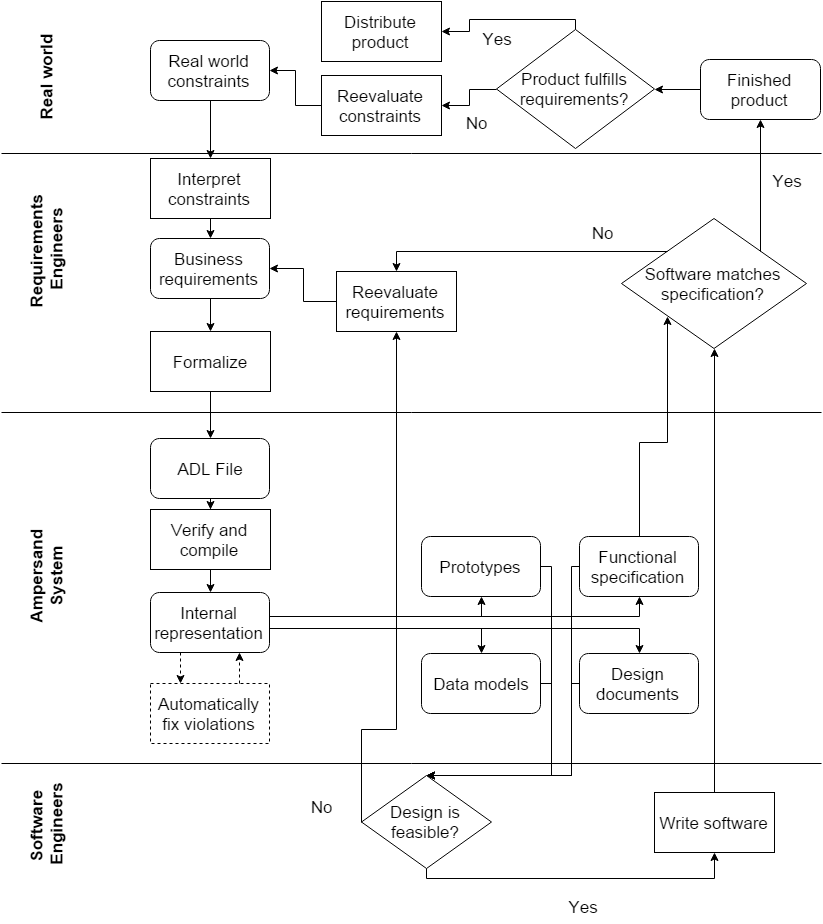
\includegraphics[width=\textwidth]{../figures/business_process}
\caption{Business process diagram representing EFA project represented as a dashed box}~\label{fig:EFAproject}
\end{center}
\end{figure}

 \subsection{The Stakeholders and the intended audience}\label{sec:Stakeholders}
The stake holders of Ampersand are:

\begin{itemize}
	\item \textbf{Ampersand Designers}: Responsible for maintaining and developing Ampersand.
	\item \textbf{The Customer}: The end users of Ampersand will benefit from the EFA project. This will decreases the amount of time 
Ampersand users spend manually inserting PHP code to restore system invariants. 
\end{itemize}

This document is designed to help introduce new Ampersand users to EFA 
(ECA rules for Ampersand). It provides a basic structure that allows 
individuals to quickly access the information they seek. 
